\chapter{図表の配置}
\label{ch:figure_table}



\section{図の配置}
\label{sec:figure}


\begin{figure}
    \centering
    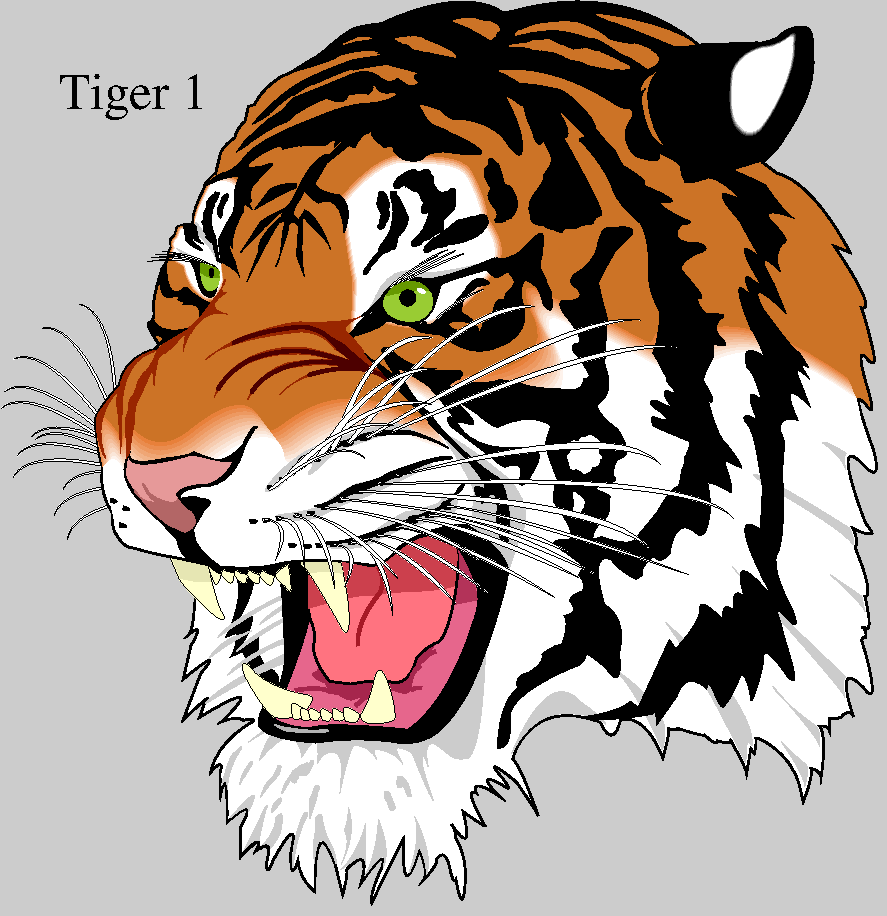
\includegraphics[width=0.5\textwidth]{figure/tiger1.pdf}
    \caption{一枚の図.}
    \label{fig:example}
\end{figure}


\begin{figure}
    \centering
    \begin{subfigure}{0.45\textwidth}
        \centering
        \includegraphics[width=\textwidth]{example-image-a}
        \caption{左の図.}
        \label{subfig:example_a}
    \end{subfigure}
    \hfill % ここで空白を入れると図が適切に配置される
    \begin{subfigure}{0.45\textwidth}
        \centering
        \includegraphics[width=\textwidth]{example-image-b}
        \caption{右の図.}
        \label{subfig:example_b}
    \end{subfigure}
    \caption{左右の図.}
    \label{fig:example2}
\end{figure}




\section{表の配置}
\label{sec:table}




